\thispagestyle{timhieukhoahocnone}
\pagestyle{timhieukhoahoc}
\everymath{\color{timhieukhoahoc}}
\blfootnote{$^1$\text{\color{timhieukhoahoc}Đại học Osnabrueck, CHLB Đức.}}
\graphicspath{{../timhieukhoahoc/pic2/}}
\begingroup
\AddToShipoutPicture*{\put(0,616){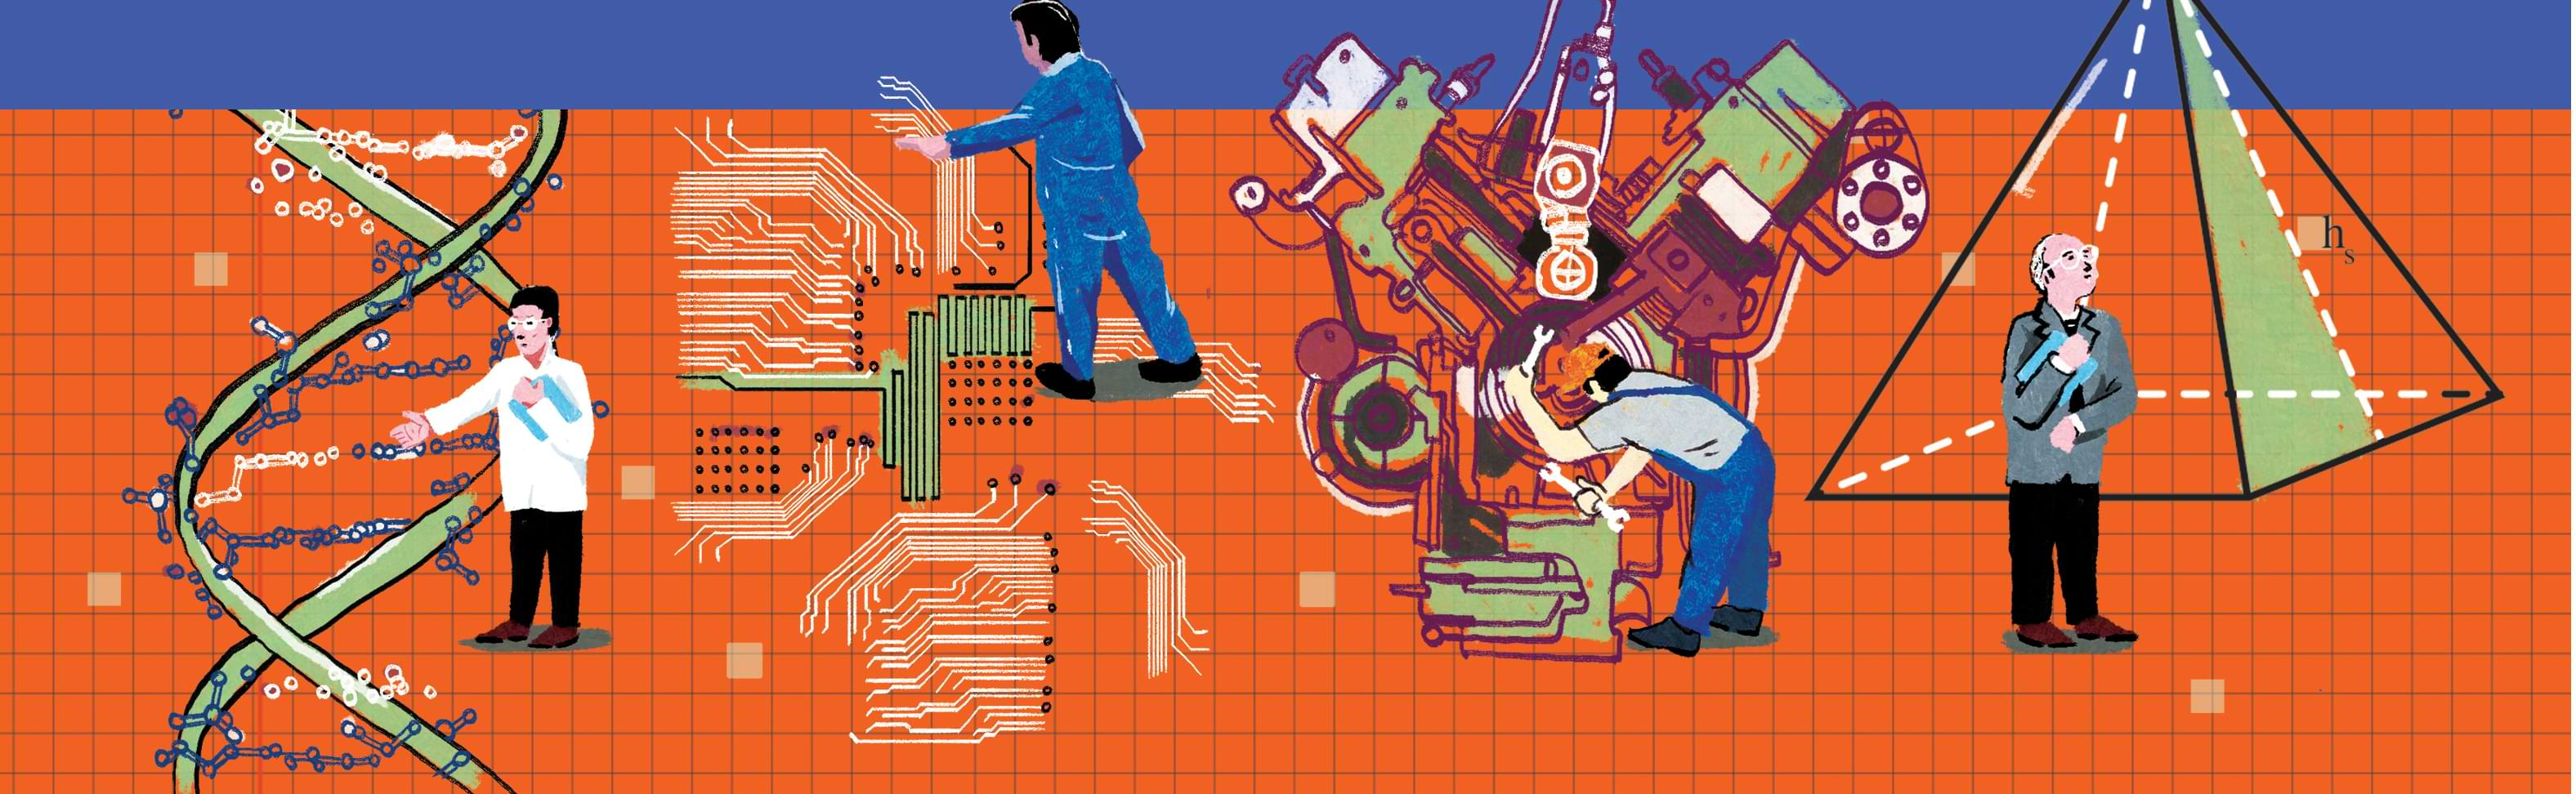
\includegraphics[width=19.3cm]{../bannertimhieu}}}
\AddToShipoutPicture*{\put(41,525){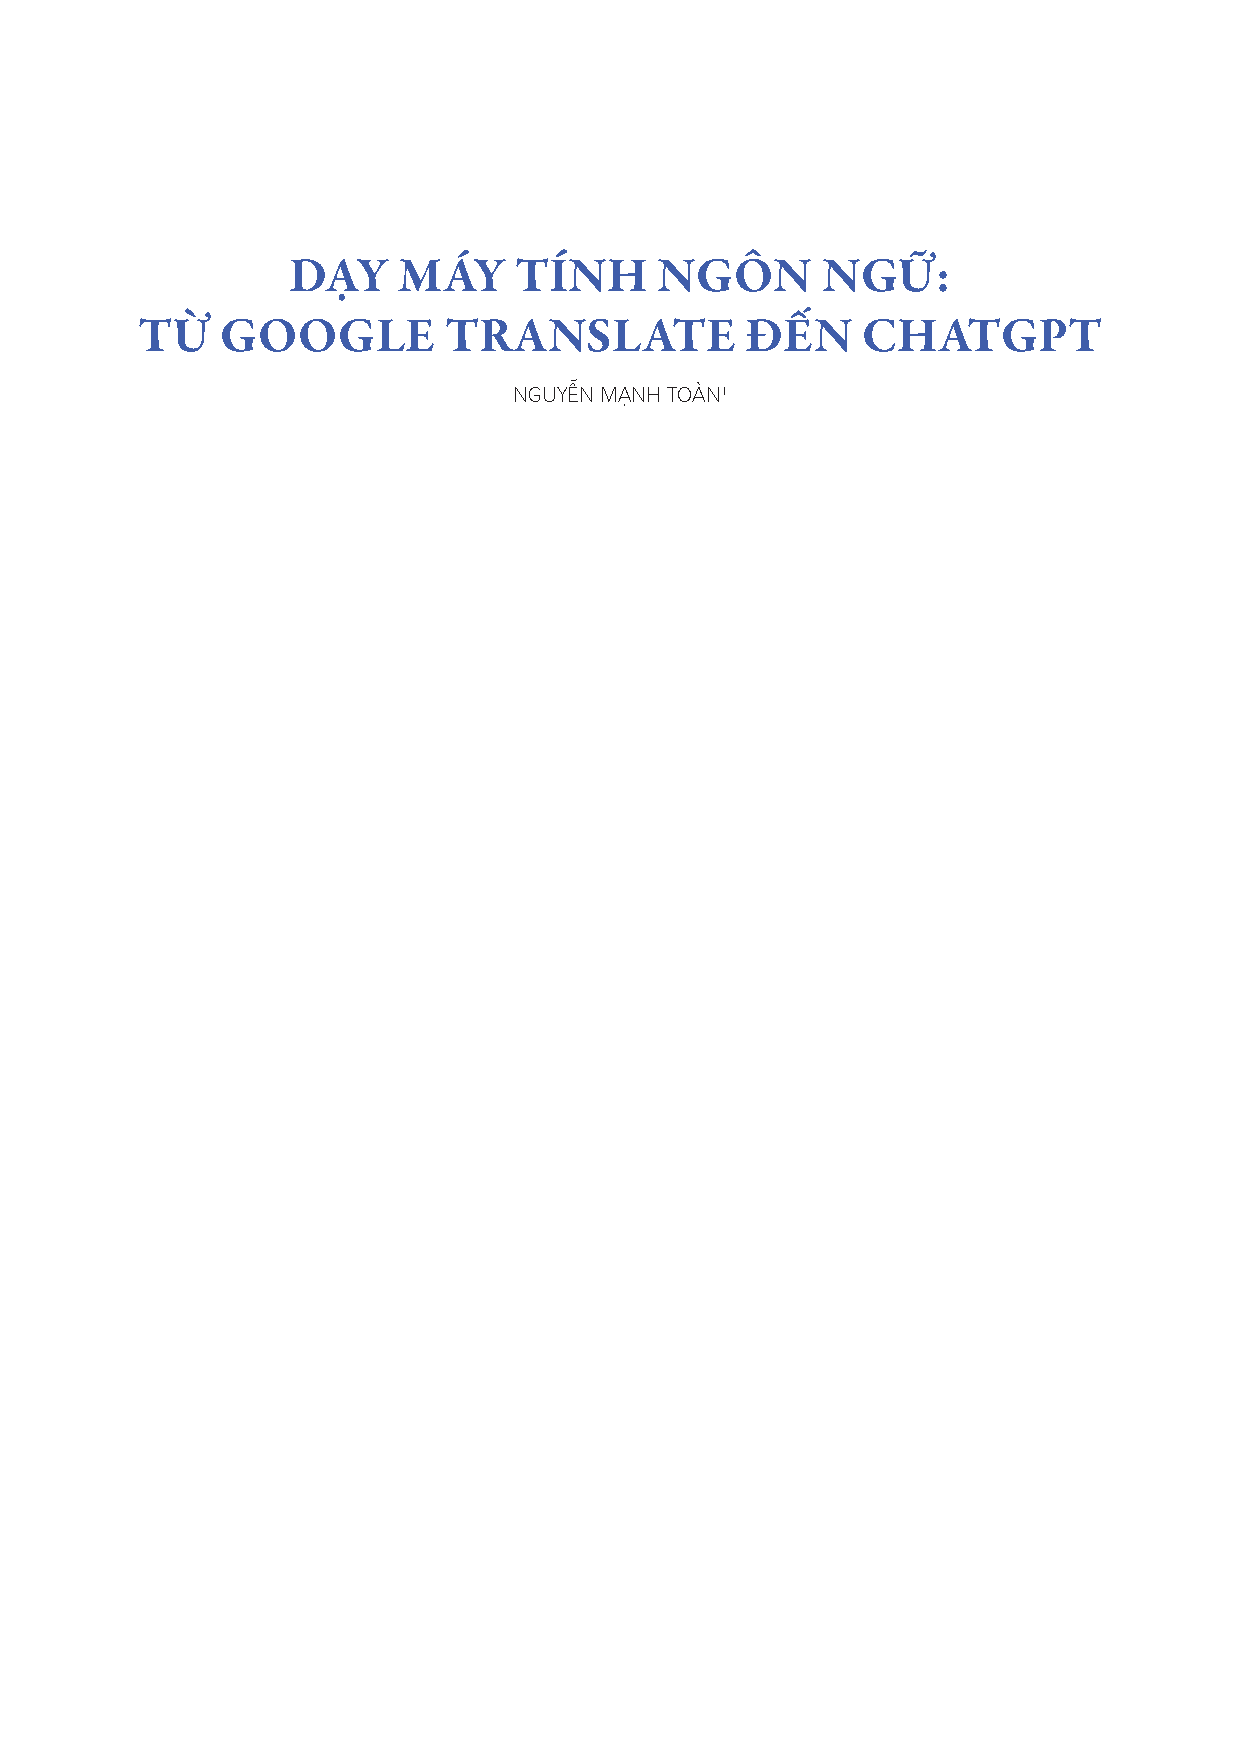
\includegraphics[scale=1]{../tieude.pdf}}}
\centering
\endgroup
\vspace*{180pt}

\begin{multicols}{2}
	\begin{figure}[H]
		\vspace*{6pt}
		\centering
		\captionsetup{labelformat= empty, justification=centering}
		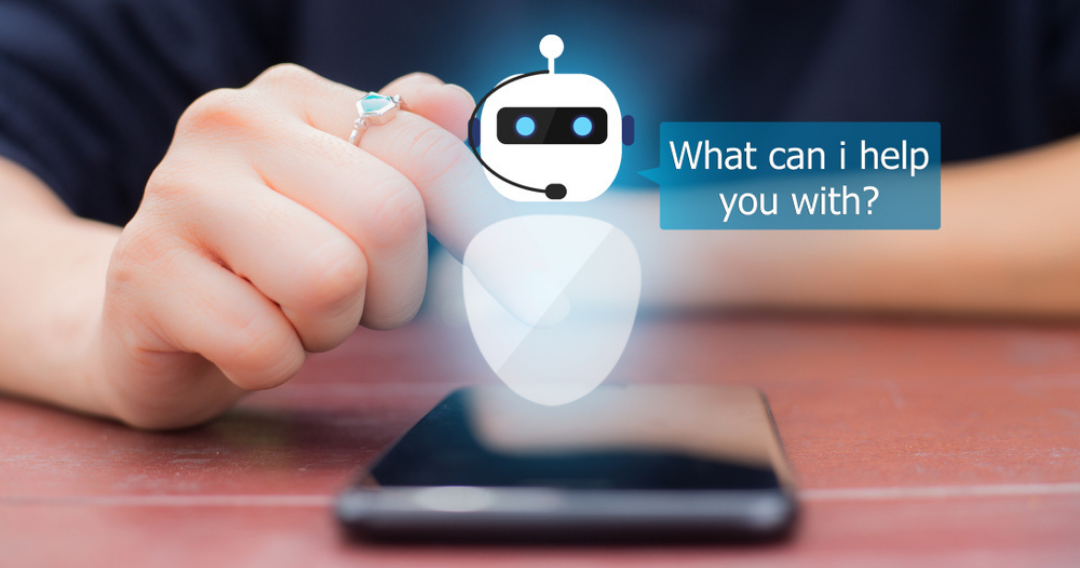
\includegraphics[width= 1\linewidth]{GPT.png}
		%		\caption{\small\textit{\color{}}}
		\vspace*{-15pt}
	\end{figure}
	\textit{Hiếm có hệ thống máy tính nào lại thu hút được nhiều sự quan tâm và tranh luận trên toàn thế giới như ChatGPT kể từ khi ra mắt vào tháng $11$ năm $2022$. Chatbot được phát triển bởi OpenAI -- một công ty công nghệ của Mỹ có trụ sở tại San Francisco -- sử dụng mô hình trí tuệ nhân tạo được đào tạo để xử lý ngôn ngữ tự nhiên. Chương trình có thể tạo ra những câu trả lời hùng hồn cho nhiều chủ đề khác nhau trong một thời gian rất ngắn, tạo ra toàn bộ bài tiểu luận hay chương trình lập trình, có thể sử dụng các phong cách ngôn ngữ như thơ, truyện cười hay thảo luận bằng các ngôn ngữ khác nhau.}
	\vskip 0.1cm
	\textit{Mặc dù bùng nổ và trở thành xu hướng chủ đạo gần như chỉ sau một đêm, ChatGPT là thành quả của nhiều thập kỷ nghiên cứu.}
	\vskip 0.1cm
	\textbf{\color{timhieukhoahoc}Một chặng đường dài}
	\vskip 0.1cm
	Vào tháng $1$ năm $1954$, một số phóng viên báo chí được lựa chọn đã tập trung trong một căn phòng lớn ở Đại học Georgetown, nơi gần như chỉ đặt một chiếc máy tính. IBM $701$ nặng gần $10$ tấn là một trong những máy tính đầu tiên được phát triển cho mục đích khoa học. Chỉ bản thân điều đó thôi đã đem đến cảm xúc cho nhiều người có mặt. Nhưng thiết bị ngoại cỡ này đã làm được một điều không thể tưởng tượng được: Khi các câu ví dụ bằng tiếng Nga được đưa vào, máy in ra bản dịch bằng tiếng Anh. Nhà ngôn ngữ học Leon Dostert, người đứng đầu dự án dịch máy Georgetown, dự đoán trong một cuộc phỏng vấn không lâu sau đó: \textit{``Trong $5$, thậm chí có thể chỉ $3$ năm nữa, việc dịch thuật đa ngôn ngữ bằng quy trình điện tử ... có thể sẽ khả thi"}. 
	\begin{figure}[H]
		\vspace*{-5pt}
		\centering
		\captionsetup{labelformat= empty, justification=centering}
		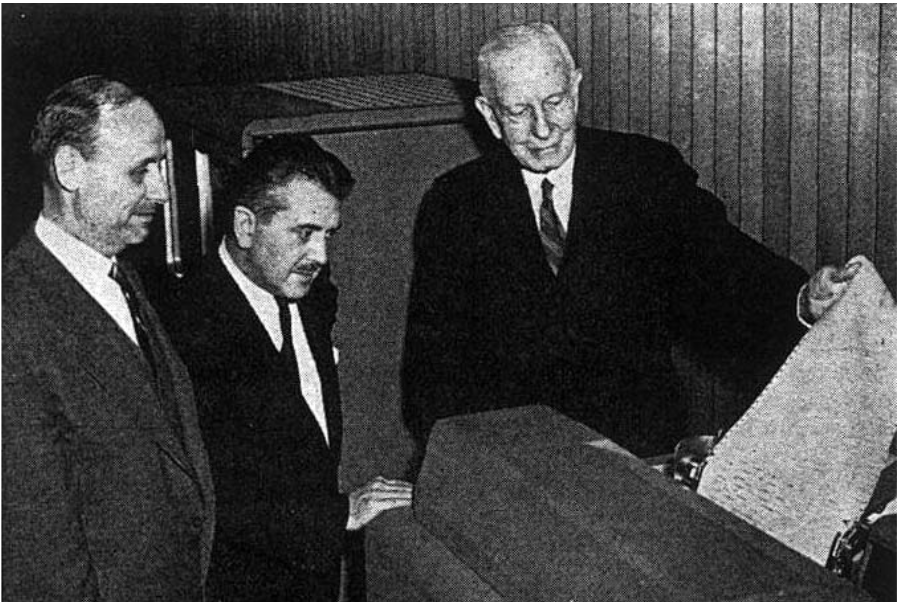
\includegraphics[width= 1\linewidth]{Georgetown-IBM.png}
		\caption{\small\textit{\color{timhieukhoahoc}Leon Dostert (giữa) và Thomas Watson (phải) -- Chủ tịch và Giám đốc điều hành của IBM -- tại buổi trình diễn của máy Georgetown.}}
		\vspace*{-5pt}
	\end{figure}
	Bây giờ chúng ta đều biết rằng Dostert đã tính toán sai những $60$ năm. Nghiên cứu về dịch máy đã phải trải qua một chặng đường rất dài. Chỉ với sự trỗi dậy gần đây của mạng thần kinh -- cuộc cách mạng học sâu -- các thuật toán học máy mới trở nên đủ mạnh để chuyển văn bản từ ngôn ngữ này sang ngôn ngữ khác một cách đáng tin cậy. 
	\vskip 0.1cm
	Nhiều cột mốc quan trọng của AI đạt được trong những năm gần đây, từ các trợ lý ảo như Siri của Apple hay Alexa của Amazon cho đến các thuật toán AI tạo sinh có khả năng tạo ra một hình ảnh hoàn toàn mới chỉ bằng một mô tả ngắn như Dall--E của OpenAI hay Stable Diffusion của StabilityAI, đều dựa vào những tiến bộ trong xử lý ngôn ngữ tự nhiên. Và có lẽ, sự ra đời của ChatGPT một năm về trước đã tạo nên làn sóng lớn nhất.
	\begin{figure}[H]
		\vspace*{-5pt}
		\centering
		\captionsetup{labelformat= empty, justification=centering}
		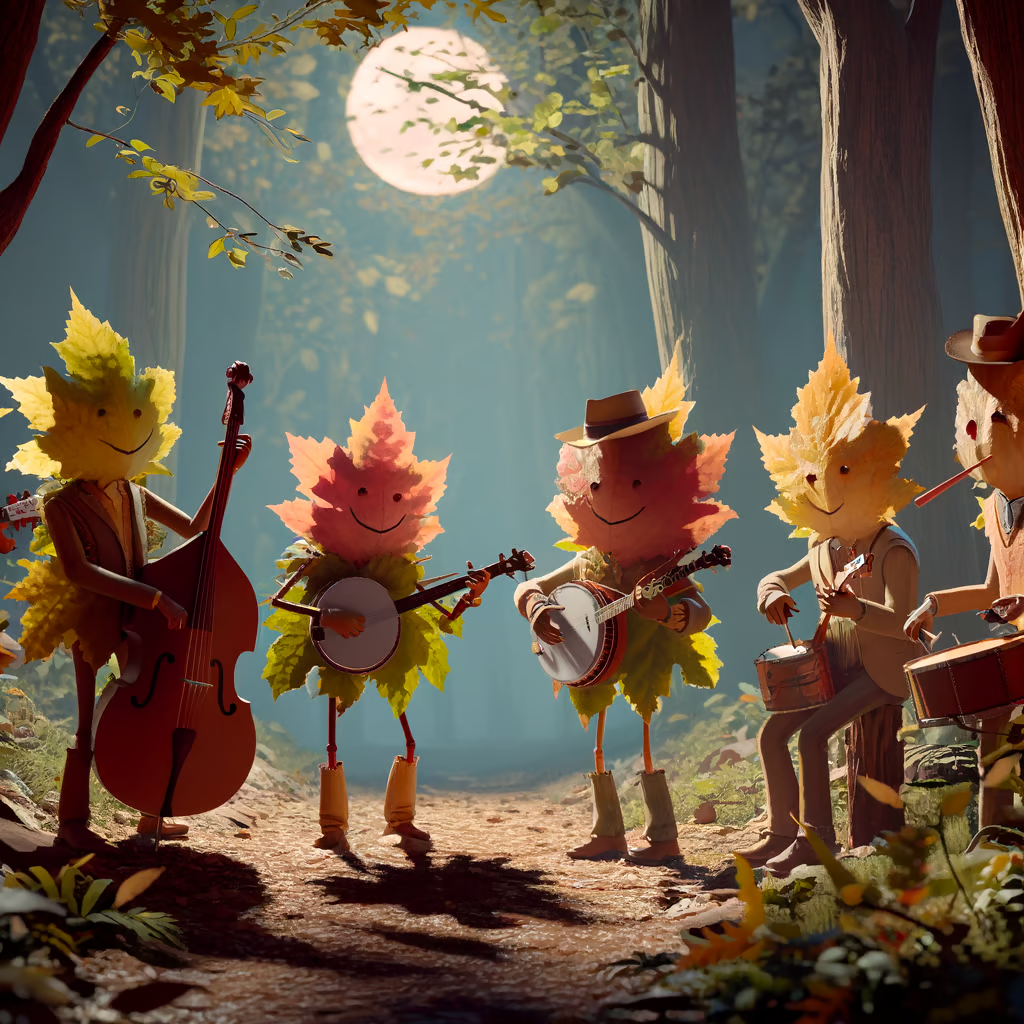
\includegraphics[width= 1\linewidth]{leaf.png}
		\caption{\small\textit{\color{timhieukhoahoc}Một bức ảnh được tạo ra bởi Dall E.}}
		\vspace*{-10pt}
	\end{figure}
	Chỉ với một câu hỏi ngắn của người dùng, ChatGPT đã có thể nhanh chóng đưa ra một đoạn giới thiệu tương đối đầy đủ về cấu trúc và khả năng của mình:
	\vskip 0.1cm
	``\textit{ChatGPT là một mô hình ngôn ngữ tự nhiên phức tạp được phát triển bởi OpenAI, dựa trên kiến trúc GPT--$3.5$. ``GPT" là viết tắt của ``Generative Pre--trained Transformer," một mô hình sử dụng kiến trúc transformer để xử lý và tạo ra văn bản. ChatGPT được đào tạo với một lượng lớn dữ liệu từ Internet, với khả năng hiểu và tạo ra văn bản tự nhiên và linh hoạt.}
	\vskip 0.1cm
	\textit{Mục tiêu chính của ChatGPT là tương tác với người dùng thông qua việc trả lời câu hỏi, thực hiện các nhiệm vụ ngôn ngữ tự nhiên và cung cấp thông tin. Nó có thể được sử dụng để hỗ trợ trong nhiều ứng dụng, bao gồm việc trả lời câu hỏi, tạo ra văn bản sáng tạo, dịch ngôn ngữ, và nhiều tác vụ ngôn ngữ khác...}"
	\vskip 0.1cm
	ChatGPT thậm chí còn có thể  sáng tạo nội dung như là kể một câu chuyện cười, điều mà ta chưa từng thấy với các chatbot trước kia:
	\vskip 0.1cm
	``\textit{Một ngày, một con gấu và một chuột đang ngồi trò chuyện. Con gấu nói, ``Bạn biết không, mỗi lần mình buồn, mình thích ăn một túi bơ."}
	\vskip 0.1cm
	\textit{Chuột nhìn con gấu và nói, ``Thực sự à? Mỗi khi tôi buồn, tôi thích ăn một thanh sô cô la."}
	\vskip 0.1cm
	\textit{Gấu ngạc nhiên và hỏi, ``Tại sao vậy?"} 
	\vskip 0.1cm
	\textit{Chuột trả lời, ``Vì sô cô la luôn giúp tôi tìm thấy mình trong tình trạng tốt hơn!"}"
	\vskip 0.1cm
	Dù nội dung có khập khiễng nhưng không thể phủ nhận rằng giờ đây chúng ta có thể giải trí một các tuyệt vời với một chương trình máy tính. AI có thể tạo ra nội dung mới như nghĩ ra những câu chuyện cười, một nghệ thuật không hề dễ dàng bởi chúng cần sự hài hước, sự đồng cảm, sự mỉa mai, sự táo bạo, v.v. Để hiểu lý do tại sao phải mất nhiều thời gian để phát triển các mô hình ngôn ngữ và những thách thức mà các nhà phát triển vẫn đang gặp phải, ta phải hiểu cách thức hoạt động của các chương trình.
	\vskip 0.1cm
	\textbf{\color{timhieukhoahoc}Nhúng từ}
	\vskip 0.1cm
	Máy tính không hiểu những mặt chữ tự nhiên thông thường như con người mà chỉ hiểu những dãy số. Do vậy, khó khăn lớn đầu tiên, cũng là điểm mấu chốt trong quá trình xử lý ngôn ngữ tự nhiên là \textit{Làm thế nào để đưa văn bản vào máy theo cách có ý nghĩa nhất có thể để tất cả các kết nối logic đều rõ ràng?} Đây là câu hỏi mà các chuyên gia đã phải vật lộn trong suốt một thời gian dài -- và vẫn đang tiếp tục phải vật lộn với nó. 
	\vskip 0.1cm
	Với hình ảnh, việc này được giải quyết tương đối dễ dàng. Ta có thể xếp các giá trị số của các điểm ảnh (pixel) lại với nhau thành một vectơ (hoặc ma trận) nhiều chiều. 
	\begin{figure}[H]
		\vspace*{-5pt}
		\centering
		\captionsetup{labelformat= empty, justification=centering}
		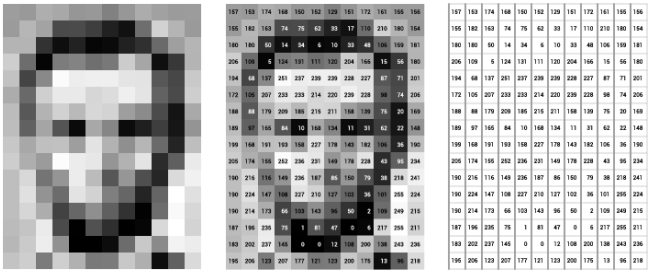
\includegraphics[width= 1\linewidth]{Computer_Vison.png}
		\caption{\small\textit{\color{timhieukhoahoc}Xử lý hình ảnh.}}
		\vspace*{-10pt}
	\end{figure}
	Tuy nhiên, với văn bản, việc gán giá trị cho từng chữ cái và dấu câu như vậy không có ý nghĩa bởi vì đối tượng thực sự mà ngôn ngữ hướng tới là từ ngữ. Việc đánh số $10.000$ mục đầu tiên trong từ điển theo thứ tự từ $1$ đến $10.000$ có thể được máy tính thực hiện dễ dàng. Tuy nhiên, điều này không giúp ích được gì bởi suy cho cùng, vấn đề không chỉ là gán các giá trị số cho nội dung mà chúng ta còn muốn các đối tượng tương tự có biểu diễn toán học không khác biệt nhiều. Với hình ảnh, khi giá trị của một vài điểm ảnh bị thay đổi thì hình ảnh được sửa đổi trông hơi khác một chút và vectơ liên quan cũng vậy. Tuy nhiên, nếu ta thực hiện những thay đổi nhỏ như là hoán đổi một chữ cái hay dấu, câu sẽ mang một ý nghĩa hoàn toàn mới. ``Con dê có bộ lông dài" khác hẳn ``con dế có bộ lông dài". Mặc dù ``dê" và ``dế" được đánh vần và viết khá giống nhau nhưng chúng khác nhau về mặt ngữ nghĩa. Trên thực tế, ``ngựa" có nhiều điểm tương đồng với ``dê" hơn dù chúng không có chung chữ cái nào.  Đó là lý do tại sao những nhà nghiên cứu về xử lý ngôn ngữ tự nhiên cần mã hóa riêng. Theo ngôn ngữ toán học, họ cần một ánh xạ để chuyển các từ có nghĩa tương tự thành các vectơ gần nhau về mặt không gian. Một ánh xạ như vậy được gọi là một \textit{Phép nhúng từ} (Word embedding).
	\begin{figure}[H]
		\vspace*{-5pt}
		\centering
		\captionsetup{labelformat= empty, justification=centering}
		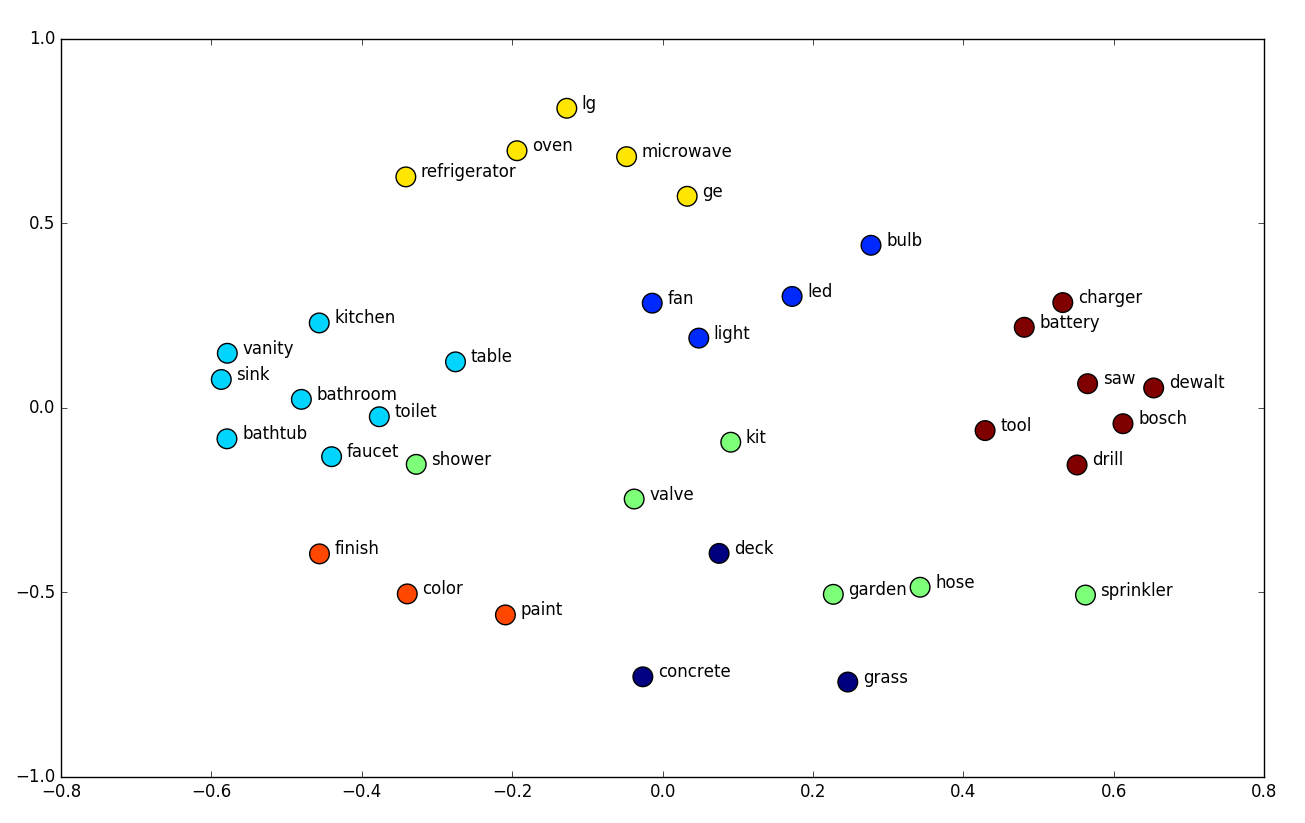
\includegraphics[width= 1\linewidth]{Word-embeddings-model.png}
		\caption{\small\textit{\color{timhieukhoahoc}Nhúng từ.}}
		\vspace*{-10pt}
	\end{figure}
	\textit{Làm thế nào để xác định khi nào hai từ giống nhau?} Theo ``giả thuyết phân phối" của Zellig Harris thì những từ có ý nghĩa tương tự sẽ xuất hiện trong những ngữ cảnh giống nhau. Dê và ngựa thường xuất hiện liên quan đến các từ như vật nuôi, lông thú, thức ăn, v.v. nên gần nghĩa, do đó sẽ được gán cho các vectơ gần nhau trong khi dê và dế có thể có khoảng cách xa hơn. 
	\vskip 0.1cm
	Trong một số trường hợp, các ràng buộc đơn giản cũng có thể được sử dụng trong phép nhúng. Chẳng hạn, hiệu của vector ``đàn ông" cho vectơ ``vua" gần với hiệu của vector ``đàn bà" cho vector ``nữ hoàng", thể hiện sự tương tự ``vua với nữ hoàng cũng như đàn ông đối với đàn bà".
	\vskip 0.1cm
	Sau khi đã tìm được phép nhúng từ phù hợp, ta sẽ biết những từ nào có thể được kết nối với nhau cũng như cách sử dụng chúng để tạo thành các câu có ý nghĩa. Do đó, cách biểu diễn thích hợp là phần quan trọng nhất của các mô hình ngôn ngữ. 
	\vskip 0.1cm
	Để tìm ra phép nhúng từ phù hợp, \textit{học máy} đã được sử dụng.\footnote[2]{\color{timhieukhoahoc}Trong nhiều thập kỷ các nhà nghiên cứu đã cố gắng áp dụng các quy tắc ngữ pháp nhưng không đem lại kết quả.} Học máy không chỉ cho phép các hệ thống "học" tự động từ dữ liệu để giải quyết những vấn đề cụ thể mà còn giúp chúng cải thiện hiệu suất theo thời gian. Mặc dù học máy bao gồm nhiều phương pháp khác nhau nhưng các kỹ thuật phổ biến nhất hiện nay đều dựa trên \textit{mạng thần kinh}.
	\vskip 0.1cm
	\textbf{\color{timhieukhoahoc}Mạng thần kinh}
	\vskip 0.1cm
	Được hình thành từ những năm $1940$ và phát triển cho đến ngày nay, mạng thần kinh là một thuật toán có cấu trúc dựa trên bộ não con người. Chúng bao gồm các đơn vị tính toán -- các \textit{nơ--ron} -- được xếp thành các lớp và các kết nối giữa chúng. Mỗi kết nối được gán cho một trọng số $w$ phù hợp. Thông tin nhận được từ nơ-ron ở đầu mỗi kết nối sẽ được nhân với trọng số  để chuyển tới nơ--ron cuối kết nối. Nơ--ron này sẽ xử lý để tạo ra thông tin mới và chuyển tới tới các nơ--ron tiếp theo. Như vậy, một mạng thần kinh là một hàm toán học đi từ tập hợp các giá trị có thể của đầu vào đến tập hợp các giá trị có thể của đầu ra.
	\begin{figure}[H]
		\vspace*{-5pt}
		\centering
		\captionsetup{labelformat= empty, justification=centering}
		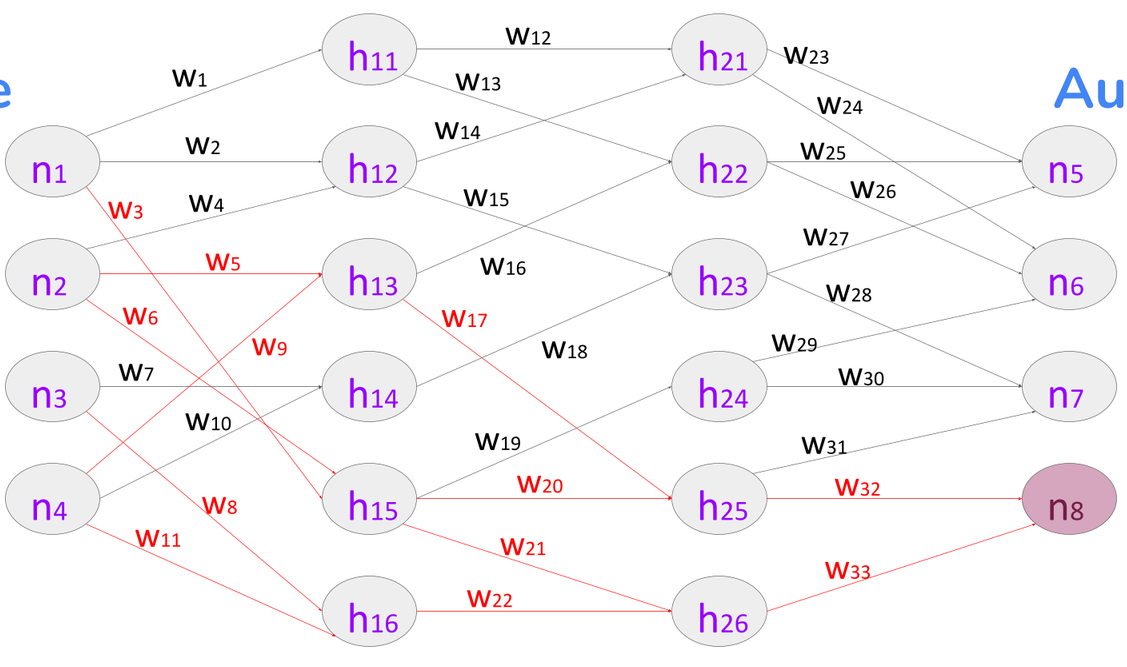
\includegraphics[width= 1\linewidth]{Neuronales_Netz1.png}
		\vspace*{-20pt}
	\end{figure}
	Nhiệm vụ bây giờ là tìm ra các giá trị phù hợp cho $w$. Với các chương trình truyền thống, lập trình viên sẽ đưa ra chỉ dẫn rõ ràng. Chẳng hạn, nếu nơ--ron $2$ từ lớp $3$ nhận được tín hiệu có giá trị $0,5$ thì hãy chuyển đổi nó thành $0,9$. Với học máy, chương trình sẽ tự tìm ra trọng số phù hợp nhất để hoàn thành nhiệm vụ. Chẳng hạn, nếu muốn mạng thần kinh nhận dạng một con vật cụ thể như ``chó" hoặc ``mèo" trong hình ảnh, ta có thể cung cấp cho mạng nhiều ví dụ mẫu. Các giá trị điểm ảnh sẽ được chuyển đến lớp đầu vào để thuật toán đưa ra kết quả dự đoán. Kết quả này sẽ được so sánh với nhãn của ảnh. Ban đầu chương trình hoạt động khá kém nhưng nó sẽ cố gắng cải thiện qua mỗi lần lặp lại. Khi đưa ra kết luận sai, chương trình sẽ điều chỉnh trọng số \footnote[3]{\color{timhieukhoahoc}Bởi có thể điều chỉnh trong quá trình đào tạo, các $w$ được gọi là \textit{tham số} của chương trình.} của các kết nối liên quan dẫn đến kết quả sai để kết quả đầu ra sẽ chính xác hơn trong tương lai. Khi chương trình liên tục tự điều chỉnh bằng cách sử dụng dữ liệu bổ sung, khả năng của nó sẽ dần được cải thiện. Khi kết thúc quá trình đào tạo, nó sẽ có thể phân loại chính xác những hình ảnh mà nó chưa từng thấy trước đây.
	\vskip 0.1cm
	Mạng thần kinh cũng có thể được sử dụng cho \textit{học không giám sát} mà ở đó các tập dữ liệu không được gắn nhãn. Chẳng hạn, ta lấy câu đầu tiên trên trang trang chủ của tạp chí Pi: ``Tạp chí Pi trực thuộc Hội Toán học Việt Nam" và chỉ chuyển một phần, chẳng hạn ``Tạp chí Pi trực thuộc ...", cho mạng thần kinh và để thuật toán dự đoán từ tiếp theo. Khi bắt đầu được đào tạo, hệ thống có thể sẽ không hoạt động tốt và tạo ra dự đoán không phù hợp. Sau đó, hệ thống sẽ điều chỉnh các tham số bên trong và từ đó cải thiện dần dần.
	\vskip 0.1cm
	Với các hệ thống dịch máy, hai mạng thần kinh thường được sử dụng là ``bộ mã hóa" và ``bộ giải mã". Bộ mã hóa thực hiện phép nhúng từ trong khi bộ giải mã tạo bản dịch từ vector biểu diễn. Với các chương trình xử lý ngôn ngữ, bộ giải mã sẽ đưa ra sự hoàn thành thích hợp nhất cho đầu vào.
	\vskip 0.1cm
	\textbf{\color{timhieukhoahoc}Mạng hồi quy}
	\vskip 0.1cm
	Không chỉ có nhiều thuật toán học máy khác nhau mà còn có nhiều loại mạng thần kinh với cấu trúc rất khác nhau. Tùy thuộc vào nhiệm vụ cần giải quyết mà ta có thể chọn, chẳng hạn như mạng thần kinh truyền tiếp (Feedforward Neural Network), mạng tích chập (Convolutional Neural Network) hay mạng hồi quy (Recurrent Neural Network). 
	\vskip 0.1cm
	Mạng thần kinh truyền tiếp là dạng đơn giản và hay gặp nhất trong đó thông tin được truyền một chiều từ đầu vào đến đầu ra. Dạng này cũng bao gồm các mạng tích chập, thường được sử dụng trong xử lý hình ảnh. Các lớp nơ-ron riêng lẻ trong mạng tích chập hoạt động giống như các bộ lọc, được sử dụng để lọc ra một số tính năng nhất định, chẳng hạn như đường viền của đối tượng được chụp ảnh. 
	\begin{figure}[H]
		\vspace*{-5pt}
		\centering
		\captionsetup{labelformat= empty, justification=centering}
		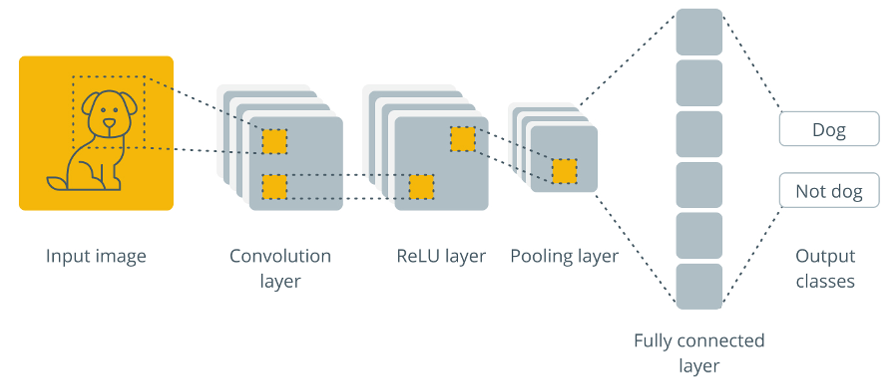
\includegraphics[width= 1\linewidth]{cnn_architecture.png}
		\caption{\small\textit{\color{timhieukhoahoc}Mạng tích chập giúp nhận diện đối tượng trong hình ảnh.}}
		\vspace*{-10pt}
	\end{figure}
	Các mạng thần kinh hồi quy chứa các vòng lặp, nơi các nơ--ron của một lớp có thể được kết nối không chỉ với các lớp tiếp theo mà còn với các nơ--ron cùng lớp hoặc các lớp trước đó. Cấu trúc này giúp xử lý dữ liệu tuần tự như là các từ trong câu một cách hiệu quả và đem lại cho các thuật toán một loại bộ nhớ, điều đặc biệt hữu ích trong việc xử lý ngôn ngữ.
	\begin{figure}[H]
		\vspace*{-5pt}
		\centering
		\captionsetup{labelformat= empty, justification=centering}
		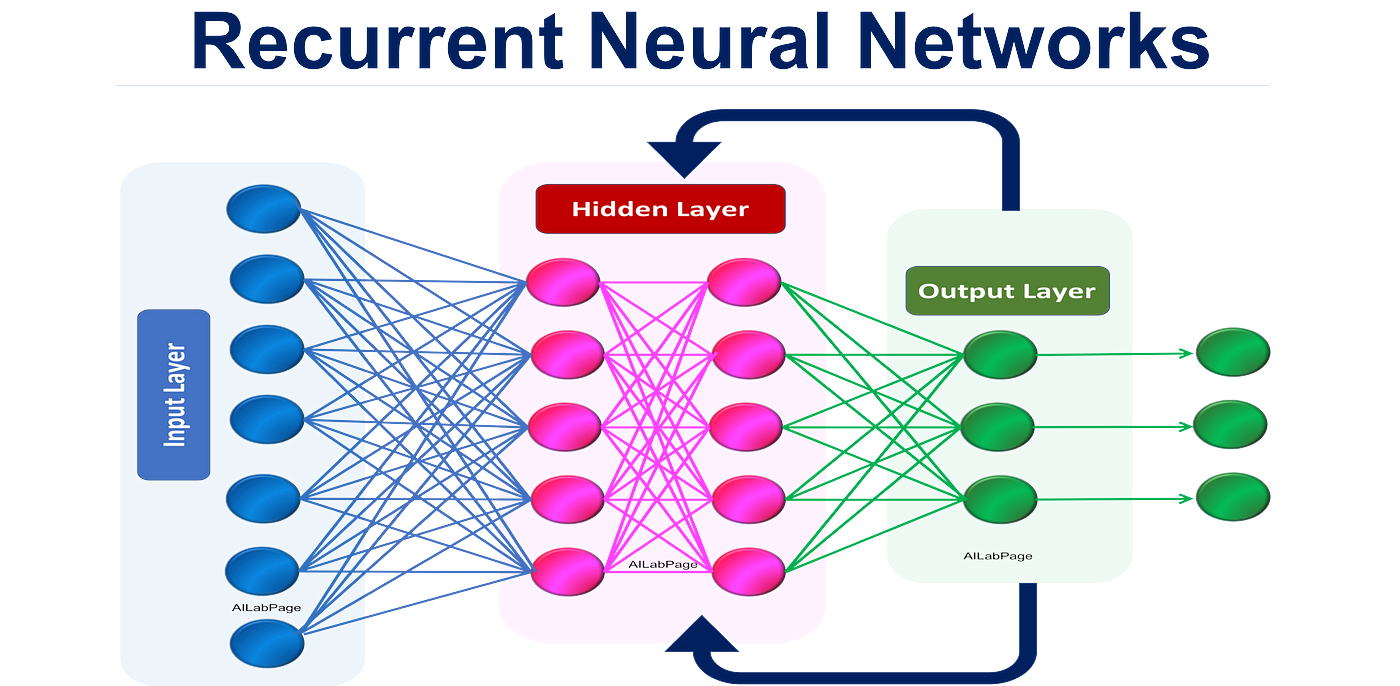
\includegraphics[width= 1\linewidth]{RNN.png}
		\caption{\small\textit{\color{timhieukhoahoc}Trong mạng nơ--ron hồi quy, thông tin không chỉ được truyền từ trái sang phải mà các lớp nơ--ron còn có thể chuyển dữ liệu sang các lớp trước đó.}}
		\vspace*{-10pt}
	\end{figure}
	Với một mạng hồi quy đã được huấn luyện trước, việc dịch một đoạn văn bản sẽ được thực hiện như thế nào? Mạng sẽ xử lý lần lượt từng từ riêng lẻ. Đầu tiên, mạng xử lý từ đầu tiên rồi lưu trữ trạng thái của các lớp bên trong dưới dạng một vector (gọi là \textit{vectơ trong}). Vector này biểu thị các tính năng liên quan của đầu vào (đó có phải là danh từ không, ngữ cảnh là gì, v.v.). Sau đó, mạng hồi quy sẽ xử lý từ thứ hai cùng với vectơ bên trong đã được tính toán trước đó. Sau đó, chương trình sẽ thay đổi vectơ bên trong, vectơ này sau đó lại được xử lý cùng với từ thứ ba, v.v. Mạng hồi quy thu thập thông tin từ nhiều nội dung bằng cách cập nhật liên tục vectơ bên trong. Khi đầu vào kết thúc, bộ mã hóa sẽ gửi vectơ này đến bộ giải mã, cuối cùng tạo đầu ra, như là hoàn thành hoặc dịch văn bản.
	\vskip 0.1cm
	Các chương trình dịch máy truyền thống như Google Translate đều hoạt động dựa trên các mạng thần kinh hồi quy. Tuy nhiên, các hệ thống này có những hạn chế: Chúng không thể xử lý đoạn văn bản dài bởi thông tin được lưu trữ trong các vectơ trong cuối cùng sẽ bị mất sau nhiều lần cập nhật. Ví dụ: nếu hai từ trong một đoạn có liên quan nhưng cách xa nhau, chương trình thường không thể nhận ra điều này. Chẳng hạn, với đoạn \textit{``Tôi sinh ra ở Việt Nam trong một làng chài nhỏ ven biển với chỉ khoảng vài chục hộ gia đình. Vì thế tôi nói trôi chảy ..."} rất có thể mạng hồi quy sẽ gặp vấn đề để hoàn thành câu vì thông tin liên quan (sinh ra ở Việt Nam) nằm ngay đầu câu đầu tiên và phải đi qua rất nhiều từ nữa mới đến khoảng trống. Đây không chỉ là trở ngại cho tạo văn bản mà còn cho dịch máy. Để dịch chính xác đại từ nhân xưng sang ngôn ngữ khác, ta phải biết chúng ám chỉ điều gì. Ngay cả khi có những thủ thuật để cải thiện thì mạng hồi quy vẫn thất bại trong việc xử lý các văn bản dài. 
	\begin{figure}[H]
		\vspace*{-5pt}
		\centering
		\captionsetup{labelformat= empty, justification=centering}
		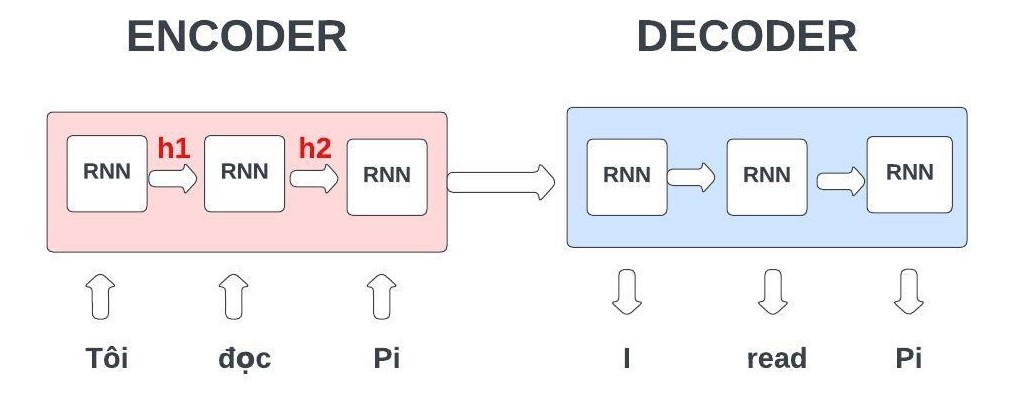
\includegraphics[width= 1\linewidth]{Encoder_Decoder.jpeg}
		\caption{\small\textit{\color{timhieukhoahoc}Dịch máy: Bộ mã hóa thu thập thông tin từ đầu vào bằng cách xử lý từng từ một, cập nhật một vectơ trong $h$ tại mỗi thời điểm. Sau đó, vectơ này được chuyển đến bộ giải mã để tạo ra một bản dịch.}}
		\vspace*{-5pt}
	\end{figure}
	Ngoài ra, bản chất tuần tự vốn có của mạng hồi quy ngăn cản việc thực hiện các tính toán một cách song song, khiến quá trình đào tạo tốn nhiều thời gian. Một máy tính chỉ có thể xử lý lần lượt từng từ trong văn bản và ta không thể tăng tốc quá trình xử lý bằng cách kết nối nhiều máy tính với nhau. 
	\vskip 0.1cm
	\textbf{\color{timhieukhoahoc}Transformer}
	\vskip 0.1cm
	Năm $2017$, một bước ngoặt lớn đã đến khi nhóm các nhà khoa học tại Google Brain xuất bản công trình \textit{Attention is all you need} (Sự chú ý là tất cả những gì bạn cần). Các tác giả tập trung vào một tính năng đặc biệt trong cách thức hoạt động của bộ não chúng ta: \textit{Sự chú ý}. Con người, may mắn thay, không chú ý đến mọi tín hiệu từ xung quanh mà chỉ tập trung sự chú ý vào những điều quan trọng đối với mình. Ví dụ, khi đang lái xe, chúng ta không quan tâm đến một chiếc lá rơi bên đường nhưng chúng ta phải phản ứng thật nhanh nếu một chiếc xe phía trước phanh gấp. Bộ não liên tục lọc các thông tin nhận được thông qua các giác quan và tập trung sự chú ý đến các tín hiệu có liên quan đến chúng ta. Các mạng Transformer cố gắng áp dụng cơ chế này -- và điều đó khiến chúng trở nên ưu việt hơn.
	\vskip 0.1cm
	Để liên kết tất cả nội dung với nhau cũng như tìm hiểu những gì được kết nối và bằng cách nào, trước tiên chương trình sẽ thực hiện phép nhúng từ cần thiết, tức chuyển từng từ riêng lẻ thành vectơ phù hợp. Sau đó, mạng sẽ tính đến các kết nối ngữ nghĩa của đầu vào và sử dụng chúng để tạo ra một biểu diễn toán học mới. Đây chính là điều khác biệt của cơ chế chú ý so với các mô hình trước đó. Để làm điều này, nhóm nghiên cứu tại Google Brain đã phát triển một phương pháp, gọi là \textit{cơ chế chú ý}, trong đó thuật toán so sánh từng từ với tất cả các từ khác và tính toán mức độ liên quan giữa chúng. 
	\vskip 0.1cm
	Chi tiết hơn, với mỗi từ trong văn bản cơ chế chú ý sẽ tính toán $3$ vector gọi là \textit{khóa}, \textit{giá trị} và \textit{truy vấn}. Sau đó các hệ số chú ý được tính toán nhằm xác định mức liên quan theo ngữ cảnh của từng tứ với các từ khác. Hệ số này là tích vô hướng của vectơ truy vấn của từ đang được xem xét với các vectơ khóa của các từ khác. Tích vô hướng đóng vai trò như thước đo mức độ ``tương tự" của hai vectơ -- do đó mức độ liên quan chặt chẽ giữa các từ. Các hệ số chú ý cho phép tạo ra cách biểu diễn mới của vector giá trị -- cách thể hiện mới của từ có tính đến nội dung của văn bản.
	\vskip 0.1cm
	Chẳng hạn ta đưa câu: ``Tôi đọc Pi vì tôi thích nó" cho thuật toán để dịch sang tiếng Anh. Chúng ta biết rằng đại từ ``nó" dùng để chỉ ``Pi". Trước tiên chương trình sẽ biến đổi mỗi từ thành một vectơ nhiều chiều. Sau đó, cơ chế chú ý xử lý từng từ trong câu: Chương trình bắt đầu bằng ``Tôi" và đặt nó trong ngữ cảnh với nội dung khác bằng cách so sánh nó với toàn bộ đầu vào, tức là ``Tôi", ``đọc", ``Pi", v.v. bằng cách tính các hệ số chú ý tương ứng. Sau đó chương trình sẽ cập nhật vector giá trị của ``Tôi".
	\begin{figure}[H]
		\vspace*{-5pt}
		\centering
		\captionsetup{labelformat= empty, justification=centering}
		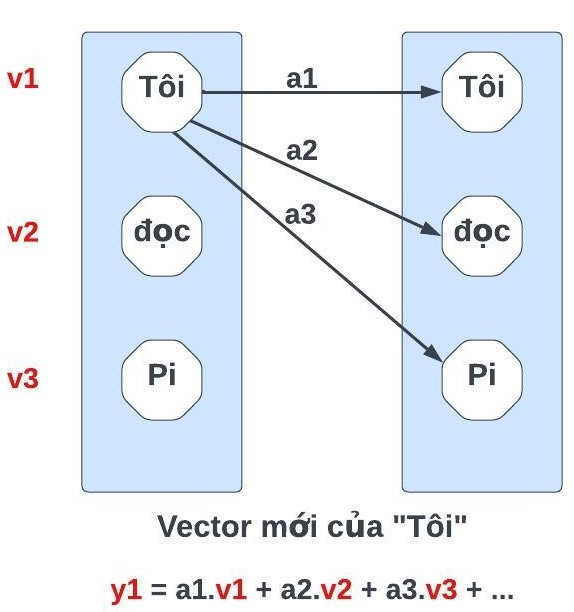
\includegraphics[width= 1\linewidth]{Attention.jpeg}
		\caption{\small\textit{\color{timhieukhoahoc}Cơ chế (tự) chú ý. Các số $a_1$, $a_2$, $a_3$, v.v. là các trọng số chú ý thể hiện mức độ liên quan của các từ đối với từ "Tôi".}}
		\vspace*{-5pt}
	\end{figure}
	Bộ mã hóa của Transformer bao gồm nhiều lớp mã hóa, mỗi lớp mã hóa bao gồm hai lớp con: một cơ chế chú ý và một mạng thần kinh truyền tiếp. Các vectơ mới thu được sau cơ chế chú ý sẽ được gửi qua mạng thần kinh tiếp nối, được biến đổi thành biểu diễn phù hợp để xử lý tiếp. Quá trình này được lặp lại nhiều lần, cho phép Transformer chú ý đến các thuộc tính ngôn ngữ khác nhau của đầu vào ở mỗi bước chú ý. Cuối cùng, bộ mã hóa tạo ra một vectơ biểu diễn cho mỗi từ trong văn bản cũng như các vectơ khóa và giá trị liên quan để bộ giải mã xử lý tiếp.
	\begin{figure}[H]
		\vspace*{-5pt}
		\centering
		\captionsetup{labelformat= empty, justification=centering}
		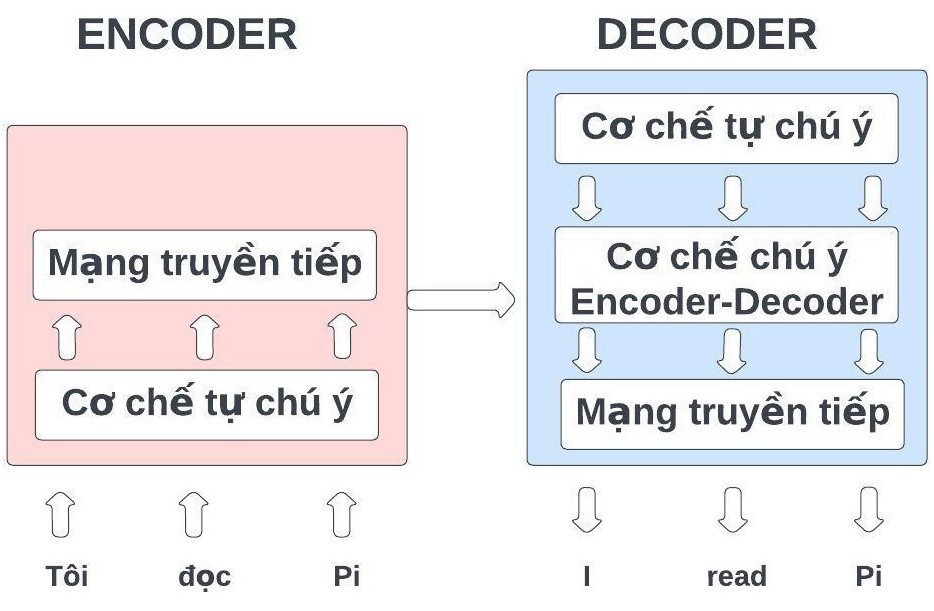
\includegraphics[width= 1\linewidth]{Transformer.jpeg}
		\caption{\small\textit{\color{timhieukhoahoc}Transformer đã cải thiện đáng kể việc xử lý ngôn ngữ bởi vì các cấu trúc sử dụng ``cơ chế chú ý" để kết nối tất cả nội dung đầu vào với nhau – bất kể khoảng cách giữa chúng.}}
		\vspace*{-10pt}
	\end{figure}
	Cũng giống như bộ mã hóa, bộ giải mã bao gồm nhiều lớp giải mã. Mỗi lớp giải mã bao gồm ba lớp con: cơ chế tự chú ý, cơ chế chú ý mã hóa-giải mã và một mạng thần kinh truyền tiếp. Tương tự như trong bộ mã hóa, cơ chế tự chú ý trong bộ giải mã cho phép Transformer xử lý các phần khác nhau trong chuỗi đầu ra, nắm bắt được sự phụ thuộc giữa các phần tử bằng cách tính toán hệ số chú ý dựa trên mối quan hệ giữa các vị trí trong chuỗi đầu ra. Cơ chế chú ý mã hóa--giải mã cho phép bộ giải mã tập trung vào các phần khác nhau của chuỗi đầu vào, kết hợp thông tin từ bộ mã hóa, chẳng hạn các từ đầu vào là tiếng nước nào. Điều này giúp bộ giải mã hiểu được ngữ cảnh của chuỗi đầu vào, hỗ trợ tạo ra chuỗi đầu ra. Mạng thần kinh truyền tiếp đưa các vectơ đã xử lý về dạng thích hợp và sau đó dịch chúng trở lại thành từ. Kết quả sau đó sẽ là một câu đúng ngữ pháp trong một ngôn ngữ khác hay một bản dịch của đầu vào.
	\vskip 0.1cm
	Với Transformer, chúng ta không phải xử lý từng từ một mà tác vụ có thể được thực hiện song song. Đơn vị tính toán có thể xác định biểu diễn vector của từ đầu tiên thông qua cơ chế chú ý, trong khi đơn vị thứ hai đồng thời dành sự chú ý cho từ thứ hai, v.v. Do vậy dữ liệu đầu vào được xử lý với Transformer nhanh hơn nhiều so với mạng thần kinh hồi quy.
	\vskip 0.1cm
	Với độ chính xác cũng như tốc độ vượt trội, Transformer đã nhanh chóng thay thế mạng thần kinh hồi quy để trở thành công nghệ tiên tiến nhất cho các nhiệm vụ xử lý ngôn ngữ. Không chỉ vậy, sự ra đời của Transformer còn thúc đẩy sự chuyển dịch mô hình trong AI khi chúng dần thay thế các mô hình học sâu truyền thống như mạng tích chập hay mạng hồi quy trong rất nhiều ứng dụng thực tiễn khác nhau.
	\vskip 0.1cm
	\textbf{\color{timhieukhoahoc}Từ dịch máy đến mô hình ngôn ngữ}
	\vskip 0.1cm
	Các mô hình ngôn ngữ như GPT (Generative Pre--Trained Transformer) của OpenAI hay BERT (Bidirectional Encoder Representations from Transformers) của Google đều sử dụng Transformer để tạo văn bản. Tuy nhiên, chúng không có cấu trúc mã hóa--giải mã như các mô hình dịch thuật mà thường chỉ sử dụng một trong hai. Chẳng hạn, các phiên bản GPT bao gồm nhiều bộ giải mã chạy nối tiếp nhau, trong khi BERT chỉ bao gồm các bộ mã hóa.
	\vskip 0.1cm
	Cơ sở cho cách tiếp cận này đến từ công trình \textit{Generating Wikipedia by Summarizing Long Sequences} (Tạo Wikipedia bằng cách tóm tắt các chuỗi dài) xuất bản năm $2018$ bởi Google Brain. Các nhà khoa học đã chỉ ra rằng ta không cần bộ mã hóa để tạo ra những văn bản có ý nghĩa. Kiến trúc chỉ dành cho bộ giải mã khá giống với các Transformer được phát triển ban đầu nhưng không yêu cầu bước chú ý thứ hai. 
	\begin{figure}[H]
		\vspace*{5pt}
		\centering
		\captionsetup{labelformat= empty, justification=centering}
		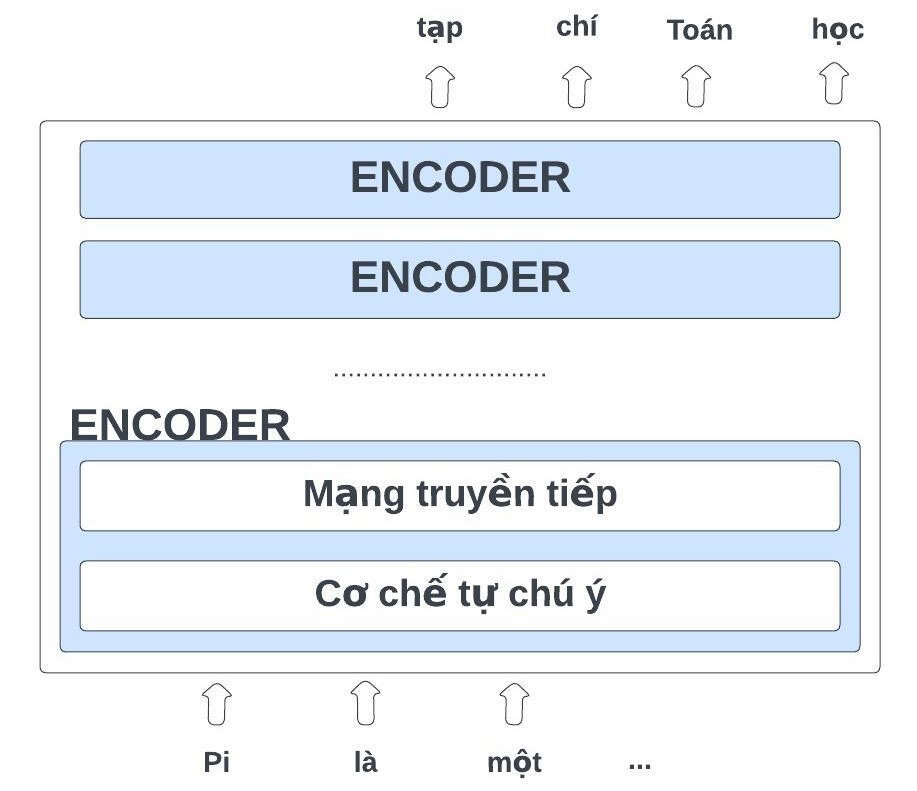
\includegraphics[width= 1\linewidth]{Decoder-Only.jpeg}
		\caption{\small\textit{\color{timhieukhoahoc}Các mô hình ngôn ngữ như GPT chỉ bao gồm bộ giải mã mà không sử dụng bộ mã hóa.}}
		\vspace*{-10pt}
	\end{figure}
	Một cách cụ thể, ta có thể cung cấp cho Transformer một đầu vào, chẳng hạn như ``Pi là một". Trước tiên thuật toán chuyển đổi đầu vào thành biểu diễn vectơ. Mỗi từ sau đó sẽ đi qua cơ chế chú ý. Bộ giải mã sẽ đánh giá tầm quan trọng của từng từ bằng cách tính toán biểu diễn vectơ mới mã hóa thông tin ngữ nghĩa quan trọng nhất. Các vector này sẽ được chuyển qua mạng truyền tiếp. Mạng này sẽ thực hiện công việc thực tế của mình là dự đoán từ nào có nhiều khả năng đi theo đầu vào nhất. 
	\vskip 0.1cm
	Đầu vào này sẽ trải qua quá trình giải mã này nhiều lần. Mỗi mạng có các trọng số khác nhau để kiểm tra các đặc điểm ngôn ngữ khác nhau của đầu vào. Cuối cùng, Transformer cung cấp một phân bố xác suất: đối với mỗi từ trong danh mục từ vựng của mình, chương trình sẽ tính toán một con số cho biết khả năng phù hợp của từ đó với đầu vào. Sau đó, Transformer chọn một trong số các từ phù hợp nhất. Chẳng hạn, đối với ``Pi là một", chương trình chọn ``tạp". Sau đó, đầu ra này được nối với đầu vào ban đầu và Transformer xử lý lại toàn bộ văn bản, tức là ``Pi là một tạp". Từ đó chương trình chọn từ tiếp theo, cụ thể là ``chí". Quá trình này tiếp tục như vậy cho đến khi kết thúc và ta nhận được: ``Pi là một tạp chí Toán học hàng tháng dành cho học sinh, sinh viên và được xuất bản bởi Hội Toán học Việt Nam."
	\vskip 0.1cm
	\textbf{\color{timhieukhoahoc}Sự phình to nhanh chóng}
	\vskip 0.1cm
	Vào tháng $6$ năm $2018$, OpenAI giới thiệu GPT--$1$, mô hình ngôn ngữ đầu tiên sử dụng Transformer. Đây cũng là hệ thống ngôn ngữ đầu tiên hoạt động tốt mà không dựa trên cơ chế học có giám sát. GPT--$1$ đã học cách xử lý ngôn ngữ tự nhiên và đưa ra các văn bản một cách thuyết phục mà không cần sự hướng dẫn của con người. Mô hình gồm $117$ triệu tham số  này được cung cấp một lượng lớn dữ liệu huấn luyện chưa được gắn nhãn. Chương trình phải sàng lọc $4,5$ Gigabyte sách chưa xuất bản và từ đó điều chỉnh các tham số. Sách đặc biệt hữu ích cho việc đào tạo các mô hình ngôn ngữ vì chúng dạy mạng thần kinh chú ý đến các kết nối ngữ nghĩa trong các đoạn văn bản dài.
	\vskip 0.1cm
	Chỉ vài tháng sau, vào tháng $2$ năm $2019$, mô hình kế nhiệm GPT--$2$ được ra mắt. Cấu trúc cơ bản của Transformer không thay đổi nhưng lượng tham số và dữ liệu huấn luyện được tăng lên $10$ lần. Các nhà phát triển đã huấn luyện mạng với $40$ Gigabyte văn bản. Lần này OpenAI đã tạo bộ dữ liệu của riêng mình. Trước tiên công ty tìm kiếm trên diễn đàn Reddit những câu trả lời phổ biến (với ít nhất ba lượt tán thành) có chứa liên kết đến các trang web và sau đó sao chép nội dung của chúng với hy vọng thu thập được thông tin chất lượng cao nhất có thể.
	\vskip 0.1cm
	Nhờ lượng dữ liệu lớn, GPT--$2$ hoạt động tốt hơn đáng kể so với phiên bản tiền nhiệm. Trên thực tế, nó tốt đến mức ban đầu OpenAI hạn chế quyền truy cập vào chương trình. Công ty không xuất bản mã nguồn đầy đủ cũng như chỉ cấp quyền sử dụng cho những người được chọn. Theo tuyên bố từ chính OpenAI, công ty lo ngại rằng công nghệ này có thể được sử dụng để tạo tin nhắn rác hoặc tin tức giả mạo. 
	\vskip 0.1cm
	Mặc dù mã nguồn không được công bố rộng rãi nhưng OpenAI đã giải thích trong một số ấn phẩm chuyên môn về các phương pháp mà họ đã sử dụng. Bởi vậy không mất nhiều thời gian để các tổ chức khác nhân rộng các mô hình ngôn ngữ tương tự. Thậm chí, hai sinh viên tại Đại học Brown là Aaron Gokaslan và Vanya Cohen có thể tái tạo lại OpenGPT--$2$ vào tháng $8$ năm $2019$. Tuy nhiên, việc triển khai không hề rẻ khi chi phí cho tính toán đào tạo có giá khoảng $50.000$ USD. Cuối cùng, sau khi nhận thấy các lo ngại về mức độ nguy hiểm của chương trình là thừa thãi, OpenAI cũng phát hành phiên bản GPT--$2$ đầy đủ ba tháng sau đó.
	\vskip 0.1cm
	Phiên bản kế nhiệm GPT--$3$ được phát hành vào tháng $6$ năm $2020$ chứa $175$ tỷ tham số và được đào tạo với khoảng $570$ Gigabyte văn bản. Mô hình này thậm chí còn tạo ra nội dung hấp dẫn hơn các phiên bản trước như có thể trả lời câu hỏi, tóm tắt tài liệu, sáng tạo câu chuyện theo nhiều phong cách khác nhau, tạo ra thuật toán bằng các ngôn ngữ lập trình khác nhau và dịch văn bản. Điều ngạc nhiên là những tiến bộ lớn này chỉ đến từ việc gia tăng dữ liệu và số tham số đào tạo. Các nguyên tắc cơ bản về kỹ thuật của GPT--$3$ vẫn không thay đổi so với các phiên bản tiền nhiệm.
	\vskip 0.1cm
	Đến tháng $3$ năm $2023$, phiên bản mới nhất, GPT--$4$, được ra mắt. Ngoài văn bản người dùng còn có đưa hình ảnh để tương tác với chương trình. Dù OpenAI từ chối tiết lộ nhiều chi tiết kỹ thuật và số liệu thống kê về GPT--$4$ nhưng theo ước tính, mô hình có khoảng có $1,76$ nghìn tỷ tham số.
	\vskip 0.1cm
	\textbf{\color{timhieukhoahoc}Phản hồi từ người dùng}
	\vskip 0.1cm
	Mặc dù GPT--$3$ cực kỳ ấn tượng -- đặc biệt là khi ta biết cách để tạo lời nhắc (Prompt) -- nhưng chương trình vẫn thể hiện những hành vi ngoài ý muốn như bịa đặt sự thật, tạo ra văn bản sai lệch, độc hại hoặc đơn giản là không tuân theo hướng dẫn của người dùng. Vì vậy, các nhà phát triển tại OpenAI đã cải tiến mô hình bằng cách sử dụng phương pháp \textit{học tăng cường từ phản hồi của con người} (Reinforcement Learning from Human Feedback) nhằm giúp mô hình đáp ứng tốt hơn các yêu cầu từ người dùng.
	\vskip 0.1cm
	Trước tiên, GPT được tinh chỉnh thông qua học tập có giám sát. Cụ thể, OpenAI thuê người viết các phản hồi mẫu cho một số lời nhắc. Tuy nhiên, chỉ một số ví dụ mà con người có thể tạo ra là không đủ để tinh chỉnh một mô hình khổng lồ với hàng tỷ tham số như GPT. Do đó, ở bước thứ hai, các chuyên gia đã tạo ra một ``mô hình phần thưởng" trong đó đầu vào của mô hình là một chuỗi lời nhắc và phản hồi, còn đầu ra là các con số, được gọi là phần thưởng: Với một lời nhắc, một số phản hồi được đưa ra. Người thử nghiệm sẽ đánh giá mức độ phù hợp của mỗi phản hồi, từ tốt nhất đến tệ nhất, và đưa ra phần thưởng tương xứng. Thông qua đó máy học được một \textit{chính sách}, tức một chiến lược để tạo ra phản hồi cho mỗi lời nhắc nhằm tối đa hóa phần thưởng. Trong bước thứ ba, GPT tạo phản hồi cho các lời nhắc và mô hình phần thưởng sẽ đánh giá kết quả. Dựa vào đánh giá đó GPT sẽ điều chỉnh các tham số nội bộ của mình để hoạt động tốt hơn trong tương lai.
	\begin{figure}[H]
		\vspace*{-5pt}
		\centering
		\captionsetup{labelformat= empty, justification=centering}
		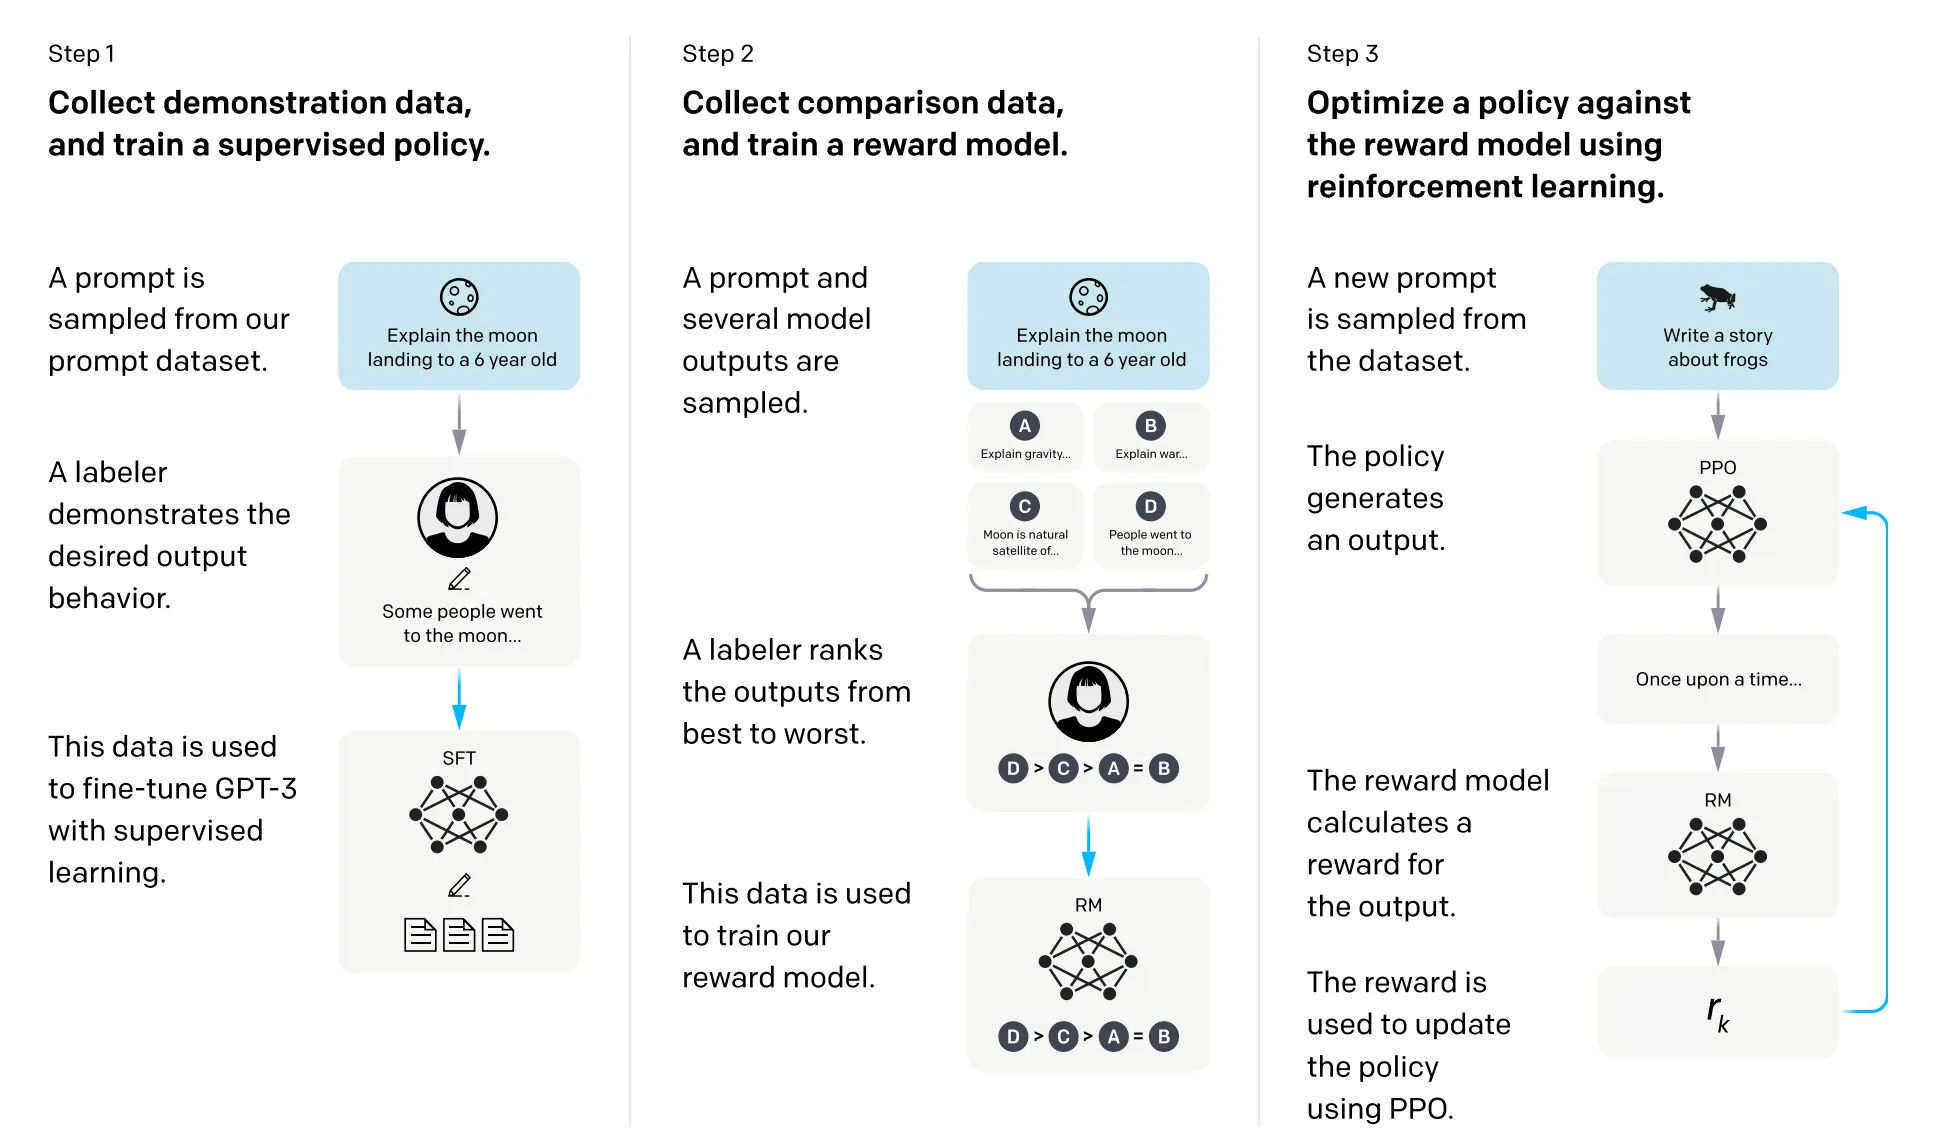
\includegraphics[width= 1\linewidth]{ChatGPT_Human_Feedback.jpeg}
		\caption{\small\textit{\color{timhieukhoahoc}Học tăng cường được sử dụng để đào tạo mô hình ngôn ngữ nhằm cung cấp câu trả lời phù hợp hơn cho các truy vấn của con người.}}
		\vspace*{-10pt}
	\end{figure}
	Hai bước cuối cùng được lặp lại nhiều lần: Sau khi GPT tự cập nhật thông qua mô hình phần thưởng, nó sẽ được đặt lại trước những đối tượng đã đánh giá kết quả đầu ra mới, tiếp tục tinh chỉnh mô hình phần thưởng. Điều này cho phép các nhà phát triển tiếp tục tinh chỉnh GPT và giới thiệu các phiên bản cải tiến cho những người thử nghiệm. Bằng cách tinh chỉnh các tham số, mô hình có thể đưa ra câu trả lời phù hợp và ít mơ hồ hơn so với các phiên bản tiền nhiệm. 
	\vskip 0.1cm
	\textbf{\color{timhieukhoahoc}ChatGPT}
	\vskip 0.1cm
	Không phải cứ mô hình lớn hơn thì sẽ ưu việt hơn. Một phiên bản cải tiến và nhỏ hơn của GPT--$3$ với chỉ với $1,3$ tỷ tham số đã hoạt động tốt hơn hệ thống đầy đủ $175$ tỷ tham số. Kết quả của những nỗ lực này sự ra đời của trợ lý trò chuyện ChatGPT vào cuối năm $2022$ và gây xôn xao kể từ đó. Chương trình này được sử dụng miễn phí và có thể thành thạo nhiều nhiệm vụ khác nhau một cách rất thuyết phục như tìm ra lỗi trong thuật toán, viết bài báo về các chủ đề hoặc trò chuyện với con người.
	\vskip 0.1cm
	Dù ChatGPT đã được tối ưu hóa để cung cấp những câu trả lời ``hài lòng nhất" có thể nhưng chương trình vẫn có những hạn chế lớn. Trước tiên, giống như các chương trình học máy khác, chất lượng đầu ra phụ thuộc vào dữ liệu được sử dụng cũng như phản hồi từ những người đào tạo chương trình. Dữ liệu khổng lồ dùng để đào tạo ChatGPT được thu thập trên web vào cuối năm $2021$, do đó chương trình không biết bất cứ điều gì được xuất bản sau đó, bao gồm nghiên cứu mới, sách hoặc sự kiện chính trị. Chẳng hạn, ChatGPT không biết rằng Nga đã tấn công Ukraine vào năm $2022$. Một hạn chế khác đến từ khả năng mắc sai lầm của con người: nếu mô hình trả lời ``Tôi không biết" cho một câu hỏi, rất có thể nó sẽ bị đánh giá kém. Vì vậy, thay vào đó, GPT bịa ra một câu trả lời thuyết phục -- câu trả lời này có thể sai nhưng được xếp hạng tốt hơn.
	\vskip 0.1cm
	Với tư cách là người dùng chúng ta cũng có thể xếp hạng kết quả đầu ra của ChatGPT. Dựa trên phản hồi này, OpenAI sẽ cải tiến mô hình. Với bản cập nhật vào tháng $2$ năm $2023$, chương trình hiện mắc ít lỗi tính toán hơn. Chẳng hạn, nếu như trước kia với câu hỏi: ``Một cây vợt và một quả bóng có giá tổng cộng là $1,10$ euro. Cây gậy đắt hơn quả bóng $1$ euro. Hỏi giá quả bóng là bao nhiêu?" chương trình sẽ đưa ra câu trả lời sai là ``$10$ xu" (câu trả lời mà mọi người thường đưa ra nhất) thì giờ đây nhờ phản hồi của con người AI đã trở nên thông minh hơn:
	\vskip 0.1cm
	{\itshape
		``Đặt giá của quả bóng là $x$ euro. Theo đó, giá của cây vợt sẽ là $x+1$ euro vì cây vợt đắt hơn quả bóng $1$ euro.
		\vskip 0.1cm
		Vậy tổng giá của cây vợt và quả bóng là $x+(x+1)=2x+1$ euro.
		\vskip 0.1cm
		Theo đề bài, tổng giá của cây vợt và quả bóng là $1,10$ euro. Vì vậy, ta có phương trình:
		\vskip 0.1cm
		$2x+1=1,10$.
		\vskip 0.1cm
		Giải phương trình này để tìm giá của quả bóng:
		\vskip 0.1cm
		$2x=0,10$
		\vskip 0.1cm
		$x=0,05$
		\vskip 0.1cm
		Vậy giá của quả bóng là 0,05 euro.}"
	\vskip 0.1cm
	\textbf{\color{timhieukhoahoc}Triển vọng và thách thức}
	\vskip 0.1cm
	Với tất cả những kết quả ấn tượng kể trên, nhiều tổ chức và tập đoàn công nghệ khác đang tìm cách đầu tư hoặc xây dựng các mô hình ngôn ngữ tương tự nhằm phục vụ cho những mục đích khác nhau. Đầu năm $2023$, Microsoft đầu tư $10$ tỷ USD vào OpenAI. Google và Facebook cũng đưa ra các mô hình ngôn ngữ của riêng mình. 
	\vskip 0.1cm
	\begin{figure}[H]
		\vspace*{-5pt}
		\centering
		\captionsetup{labelformat= empty, justification=centering}
		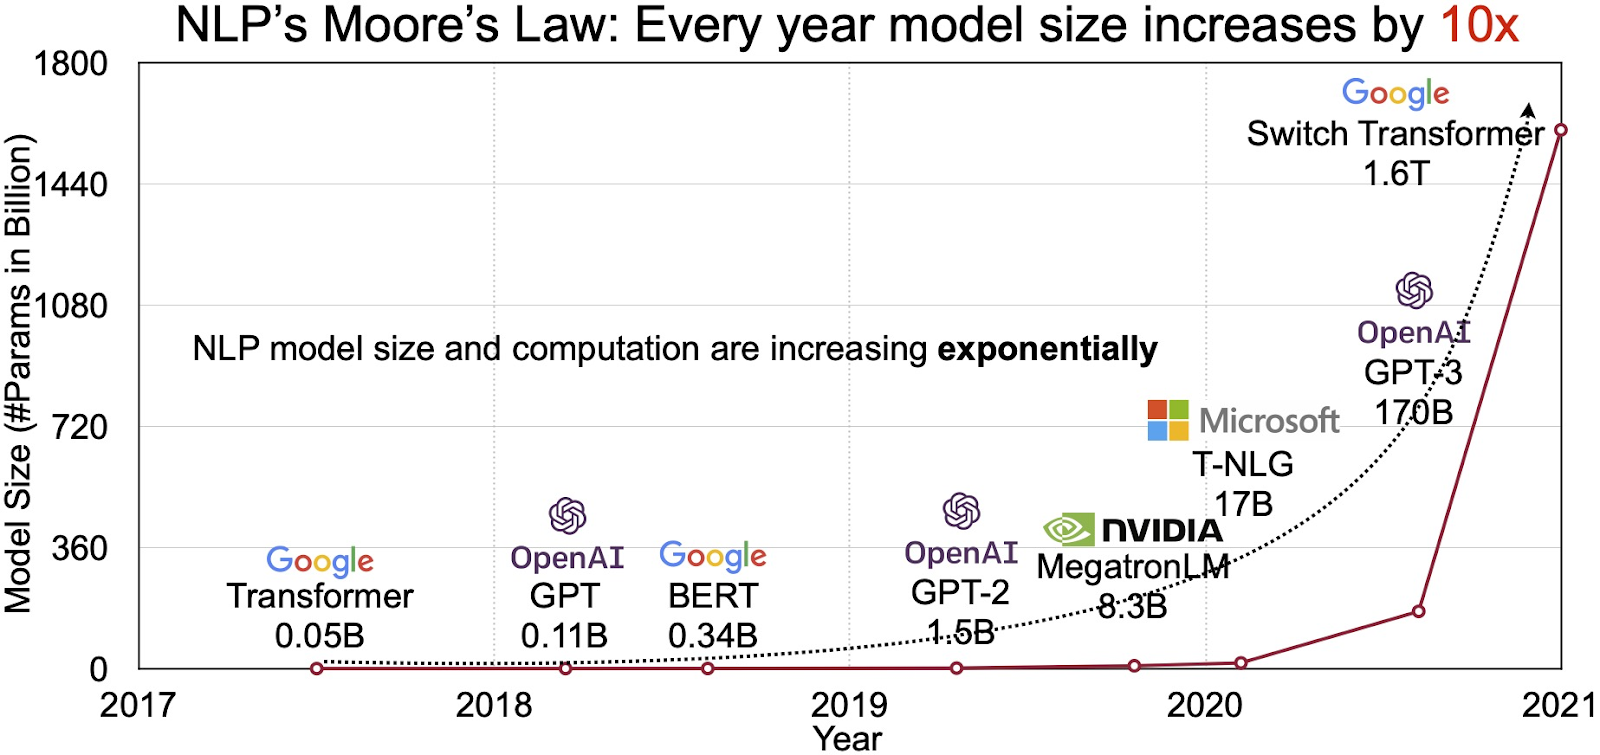
\includegraphics[width= 1\linewidth]{MooreAI.png}
		\caption{\small\textit{\color{timhieukhoahoc}Kích thước các mô hình ngôn ngữ.}}
		\vspace*{-10pt}
	\end{figure}
	Không chỉ giới hạn trong việc dịch ngôn ngữ và tạo nội dung, các mô hình ngôn ngữ lớn được sử dụng rộng rãi trong rất nhiều lĩnh vực khác nhau, từ phát hiện và ngăn chặn các cuộc tấn công mạng cho đến nghiên cứu thị trường, tự động hóa bán hàng, phân tích quan điểm, học tập và nghiên cứu, thậm chí là giải quyết các vấn đề mở trong toán học. Trong công trình vừa xuất bản trên tạp chí \textit{Nature} ngày $14.12.2023$ vừa qua, các nhà khoa học tại Google DeepMind đã sử dụng một mô hình ngôn ngữ lớn gọi là FunSearch để giải quyết một bài toán nổi tiếng thuộc lĩnh vực tổ hợp. 
	\vskip 0.1cm
	Mặc dù là một nguồn lực mới mà bất cứ quốc gia hay doanh nghiệp nào cũng muốn sở hữu nhưng các mô hình ngôn ngữ cũng đặt ra những vấn đề và thách thức không dễ để giải quyết. 
	\vskip 0.1cm
	Trước hết là vấn đề bảo mật và quyền riêng tư. Các mô hình ngôn ngữ lớn cần quyền truy cập vào lượng lớn dữ liệu văn bản để đào tạo, gây ra những lo ngại về quyền riêng tư, chủ yếu là khi xử lý thông tin nhạy cảm hoặc bí mật. Việc bảo vệ dữ liệu người dùng và tuân thủ các quy định bảo vệ dữ liệu là rất cần thiết trong bối cảnh này. Bên cạnh đó, chính phủ và các nhà khoa học lo ngại việc sẽ mất chủ quyền nếu giao toàn bộ dữ liệu của mình, đặc biệt là thông tin nội bộ công ty, cho một công ty Mỹ. 
	\vskip 0.1cm
	Một số chuyên gia cũng nêu lên mối lo ngại về tác động môi trường của việc đào tạo các mô hình ngôn ngữ lớn như GPT, vốn đòi hỏi một lượng lớn năng lượng và sức mạnh tính toán. Theo các nhà nghiên cứu của đại học Massachusetts, việc đào tạo mô hình BERT của Google trên GPU tạo ra lượng khí thải gần tương đương với một chuyến bay xuyên Mỹ. Google cũng cho biết việc đào tạo mô hình ngôn ngữ PaLM của họ sử dụng năng lượng tương đương với $300$ hộ gia đình ở Mỹ trong một năm. 
	\vskip 0.1cm
	Thêm vào đó, chi phí xây dựng cơ sở hạ tầng cho các mô hình ngôn ngữ rất đắt đỏ. Theo Sam Altman -- đồng sáng lập và giám đốc điều hành của OpenAI -- trong một bài phỏng vấn vào tháng $7$ vừa qua thì chi phí đào tạo các mô hình cơ bản hiện nay không dưới $100$ triệu USD. Theo ước tính từ một số chuyên gia, chi phí đào tạo thế hệ mô hình ngôn ngữ lớn tiếp theo sẽ vượt qua $1$ tỷ USD trong vòng vài năm tới. Ngoài ra, các mô hình ngôn ngữ lớn đòi hỏi những kho liệu khổng lồ để đào tạo. Để có thể sử dụng các mô hình ngôn ngữ cho mục đích thương mại, những kho dữ liệu thương mại cần phải được xây dựng. Điều này đòi hỏi rất nhiều tiền bạc, công sức và thời gian. 
	\vskip 0.1cm
	\textbf{\color{timhieukhoahoc}Tài liệu tham khảo}
	\vskip 0.1cm
	[$1$] Vaswani, A. et al. \textit{Attention is all you need.} Advances in neural information processing systems ($2017$).
	\vskip 0.1cm
	[$2$] Liu, P. et al. \textit{Generating Wikipedia by Summarizing Long Sequences}. International Conference on Learning Representations ($2018$).
	\vskip 0.1cm
	[$3$] Ouyang, L. et al. \textit{Training language models to follow instructions with human feedback}. \url{arxiv.org/abs/2203.02155}
	\vskip 0.1cm
	[$4$] Romera--Paredes, B. et al. \textit{Mathematical discoveries from program search with large language models}. Nature ($2023$).
\end{multicols}


